\documentclass[twoside]{book}

% Packages required by doxygen
\usepackage{fixltx2e}
\usepackage{calc}
\usepackage{doxygen}
\usepackage[export]{adjustbox} % also loads graphicx
\usepackage{graphicx}
\usepackage[utf8]{inputenc}
\usepackage{makeidx}
\usepackage{multicol}
\usepackage{multirow}
\PassOptionsToPackage{warn}{textcomp}
\usepackage{textcomp}
\usepackage[nointegrals]{wasysym}
\usepackage[table]{xcolor}

% Font selection
\usepackage[T1]{fontenc}
\usepackage[scaled=.90]{helvet}
\usepackage{courier}
\usepackage{amssymb}
\usepackage{sectsty}
\renewcommand{\familydefault}{\sfdefault}
\allsectionsfont{%
  \fontseries{bc}\selectfont%
  \color{darkgray}%
}
\renewcommand{\DoxyLabelFont}{%
  \fontseries{bc}\selectfont%
  \color{darkgray}%
}
\newcommand{\+}{\discretionary{\mbox{\scriptsize$\hookleftarrow$}}{}{}}

% Page & text layout
\usepackage{geometry}
\geometry{%
  a4paper,%
  top=2.5cm,%
  bottom=2.5cm,%
  left=2.5cm,%
  right=2.5cm%
}
\tolerance=750
\hfuzz=15pt
\hbadness=750
\setlength{\emergencystretch}{15pt}
\setlength{\parindent}{0cm}
\setlength{\parskip}{3ex plus 2ex minus 2ex}
\makeatletter
\renewcommand{\paragraph}{%
  \@startsection{paragraph}{4}{0ex}{-1.0ex}{1.0ex}{%
    \normalfont\normalsize\bfseries\SS@parafont%
  }%
}
\renewcommand{\subparagraph}{%
  \@startsection{subparagraph}{5}{0ex}{-1.0ex}{1.0ex}{%
    \normalfont\normalsize\bfseries\SS@subparafont%
  }%
}
\makeatother

% Headers & footers
\usepackage{fancyhdr}
\pagestyle{fancyplain}
\fancyhead[LE]{\fancyplain{}{\bfseries\thepage}}
\fancyhead[CE]{\fancyplain{}{}}
\fancyhead[RE]{\fancyplain{}{\bfseries\leftmark}}
\fancyhead[LO]{\fancyplain{}{\bfseries\rightmark}}
\fancyhead[CO]{\fancyplain{}{}}
\fancyhead[RO]{\fancyplain{}{\bfseries\thepage}}
\fancyfoot[LE]{\fancyplain{}{}}
\fancyfoot[CE]{\fancyplain{}{}}
\fancyfoot[RE]{\fancyplain{}{\bfseries\scriptsize Generated by Doxygen }}
\fancyfoot[LO]{\fancyplain{}{\bfseries\scriptsize Generated by Doxygen }}
\fancyfoot[CO]{\fancyplain{}{}}
\fancyfoot[RO]{\fancyplain{}{}}
\renewcommand{\footrulewidth}{0.4pt}
\renewcommand{\chaptermark}[1]{%
  \markboth{#1}{}%
}
\renewcommand{\sectionmark}[1]{%
  \markright{\thesection\ #1}%
}

% Indices & bibliography
\usepackage{natbib}
\usepackage[titles]{tocloft}
\setcounter{tocdepth}{3}
\setcounter{secnumdepth}{5}
\makeindex

% Hyperlinks (required, but should be loaded last)
\usepackage{ifpdf}
\ifpdf
  \usepackage[pdftex,pagebackref=true]{hyperref}
\else
  \usepackage[ps2pdf,pagebackref=true]{hyperref}
\fi
\hypersetup{%
  colorlinks=true,%
  linkcolor=blue,%
  citecolor=blue,%
  unicode%
}

% Custom commands
\newcommand{\clearemptydoublepage}{%
  \newpage{\pagestyle{empty}\cleardoublepage}%
}

\usepackage{caption}
\captionsetup{labelsep=space,justification=centering,font={bf},singlelinecheck=off,skip=4pt,position=top}

%===== C O N T E N T S =====

\begin{document}

% Titlepage & ToC
\hypersetup{pageanchor=false,
             bookmarksnumbered=true,
             pdfencoding=unicode
            }
\pagenumbering{alph}
\begin{titlepage}
\vspace*{7cm}
\begin{center}%
{\Large On\+Eg\+IN }\\
\vspace*{1cm}
{\large Generated by Doxygen 1.8.13}\\
\end{center}
\end{titlepage}
\clearemptydoublepage
\pagenumbering{roman}
\tableofcontents
\clearemptydoublepage
\pagenumbering{arabic}
\hypersetup{pageanchor=true}

%--- Begin generated contents ---
\chapter{Evgeniy Onegin sorter}
\label{index}\hypertarget{index}{}~\newline
Usage\+: ./\+On\+Eg\+IN \mbox{[}-\/param\mbox{]} \mbox{[}input.\+file\mbox{]} \mbox{[}output.\+file\mbox{]} ~\newline
Params\+: \mbox{[}-\/l\mbox{]}\+: compare lexigraphically; \mbox{[}-\/r\mbox{]}\+: compare rythmically ~\newline
Example\+: ./\+On\+Eg\+IN -\/r onegin.\+txt onegin\+Sorted\+\_\+rythms.\+txt ~\newline
\begin{DoxyAuthor}{Author}
Titov.\+EM ~\newline
Files\+: ~\newline

\begin{DoxyItemize}
\item \hyperlink{main_8cpp}{main.\+cpp} ~\newline
 
\end{DoxyItemize}
\end{DoxyAuthor}

\chapter{Class Index}
\section{Class List}
Here are the classes, structs, unions and interfaces with brief descriptions\+:\begin{DoxyCompactList}
\item\contentsline{section}{\hyperlink{unionwch}{wch} }{\pageref{unionwch}}{}
\end{DoxyCompactList}

\chapter{File Index}
\section{File List}
Here is a list of all files with brief descriptions\+:\begin{DoxyCompactList}
\item\contentsline{section}{\hyperlink{main_8cpp}{main.\+cpp} }{\pageref{main_8cpp}}{}
\end{DoxyCompactList}

\chapter{Class Documentation}
\hypertarget{unionwch}{}\section{wch Union Reference}
\label{unionwch}\index{wch@{wch}}
\subsection*{Public Attributes}
\begin{DoxyCompactItemize}
\item 
char \hyperlink{unionwch_af55b442864f410a46904f7fb15c1ca3a}{sym} \mbox{[}2\mbox{]}
\item 
unsigned int \hyperlink{unionwch_aa8de173ef97cc017c30e24819ab3a10a}{dig}
\end{DoxyCompactItemize}


\subsection{Detailed Description}


Definition at line 166 of file main.\+cpp.



\subsection{Member Data Documentation}
\mbox{\Hypertarget{unionwch_aa8de173ef97cc017c30e24819ab3a10a}\label{unionwch_aa8de173ef97cc017c30e24819ab3a10a}} 
\index{wch@{wch}!dig@{dig}}
\index{dig@{dig}!wch@{wch}}
\subsubsection{\texorpdfstring{dig}{dig}}
{\footnotesize\ttfamily unsigned int wch\+::dig}



Definition at line 168 of file main.\+cpp.

\mbox{\Hypertarget{unionwch_af55b442864f410a46904f7fb15c1ca3a}\label{unionwch_af55b442864f410a46904f7fb15c1ca3a}} 
\index{wch@{wch}!sym@{sym}}
\index{sym@{sym}!wch@{wch}}
\subsubsection{\texorpdfstring{sym}{sym}}
{\footnotesize\ttfamily char wch\+::sym\mbox{[}2\mbox{]}}



Definition at line 167 of file main.\+cpp.



The documentation for this union was generated from the following file\+:\begin{DoxyCompactItemize}
\item 
\hyperlink{main_8cpp}{main.\+cpp}\end{DoxyCompactItemize}

\chapter{File Documentation}
\hypertarget{main_8cpp}{}\section{main.\+cpp File Reference}
\label{main_8cpp}\index{main.\+cpp@{main.\+cpp}}
{\ttfamily \#include $<$stdio.\+h$>$}\newline
{\ttfamily \#include $<$stdlib.\+h$>$}\newline
{\ttfamily \#include $<$string.\+h$>$}\newline
{\ttfamily \#include $<$ctype.\+h$>$}\newline
{\ttfamily \#include $<$locale.\+h$>$}\newline
{\ttfamily \#include $<$assert.\+h$>$}\newline
{\ttfamily \#include $<$sys/stat.\+h$>$}\newline
Include dependency graph for main.\+cpp\+:\nopagebreak
\begin{figure}[H]
\begin{center}
\leavevmode
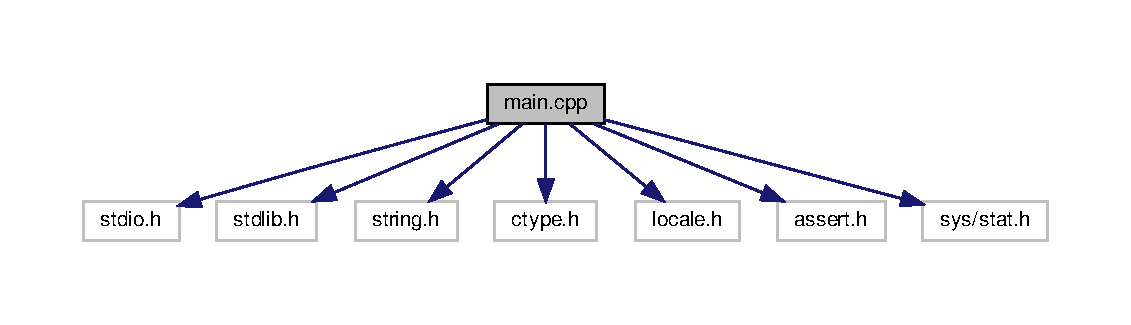
\includegraphics[width=350pt]{main_8cpp__incl}
\end{center}
\end{figure}
\subsection*{Classes}
\begin{DoxyCompactItemize}
\item 
union \hyperlink{unionwch}{wch}
\end{DoxyCompactItemize}
\subsection*{Macros}
\begin{DoxyCompactItemize}
\item 
\#define \hyperlink{main_8cpp_a944fe8428680f2d017c129adede0fae9}{C\+H\+E\+C\+K\+\_\+\+S\+T\+R\+\_\+\+E\+ND}(x,  y)
\item 
\#define \hyperlink{main_8cpp_a5514670076404ebe732e1c84bafd9248}{R\+E\+V\+E\+R\+SE}(x,  y)
\end{DoxyCompactItemize}
\subsection*{Functions}
\begin{DoxyCompactItemize}
\item 
long long \hyperlink{main_8cpp_aef860ff26bf8fabdb8c0288cf07bf71f}{get\+\_\+file\+\_\+size\+\_\+\+L\+I\+N\+UX} (char $\ast$filename)
\item 
long \hyperlink{main_8cpp_a188b0b992185dc36cb540859f083ccde}{get\+\_\+lines\+\_\+\+N\+UM} (F\+I\+LE $\ast$file, long long Fsize)
\item 
int \hyperlink{main_8cpp_a84ee31895c6ea98147787569aa984847}{M\+A\+S\+\_\+read} (F\+I\+LE $\ast$file, long long Fsize, char $\ast$mas, char $\ast$$\ast$pointers)
\item 
int \hyperlink{main_8cpp_a1cb3b8b80beaf62114f3f2bc01fa2bb4}{M\+A\+S\+\_\+write} (char $\ast$$\ast$pointers, F\+I\+LE $\ast$file, long long num)
\item 
int \hyperlink{main_8cpp_afd6f42e0e484cd684e773edf5b848b3e}{fopen\+\_\+\+IO} (char $\ast$file\+Name1, char $\ast$file\+Name2, F\+I\+LE $\ast$$\ast$in, F\+I\+LE $\ast$$\ast$out)
\item 
int \hyperlink{main_8cpp_aeefefe84c8959c242dd6066132c7db5b}{tolowerstr} (char $\ast$str)
\item 
int \hyperlink{main_8cpp_a267fcfc60a3469cd3946335bac2c45f1}{strcheck} (char $\ast$str)
\item 
int \hyperlink{main_8cpp_ab44933387b50247a5767d00459953984}{compstr} (const void $\ast$a, const void $\ast$b)
\item 
int \hyperlink{main_8cpp_a732094ae997dd915b27ca6b615421d4b}{chcheck} (char ch)
\item 
int \hyperlink{main_8cpp_ac979745969e12b24f262b443fc2f118d}{strcmp\+\_\+lecs} (char $\ast$str1, char $\ast$str2)
\item 
int \hyperlink{main_8cpp_aa81366f7c2b1030b2f59ed847c997a6c}{strcmp\+\_\+rythms\+\_\+utf8} (char $\ast$str1, char $\ast$str2)
\item 
int \hyperlink{main_8cpp_a0ddf1224851353fc92bfbff6f499fa97}{main} (int argc, char $\ast$argv\mbox{[}$\,$\mbox{]})
\end{DoxyCompactItemize}
\subsection*{Variables}
\begin{DoxyCompactItemize}
\item 
int \hyperlink{main_8cpp_ac56e9668908c973d5f99b446a5144ecb}{B\+E\+H\+A\+V\+I\+OR} = 0
\begin{DoxyCompactList}\small\item\em Defines program behavior\+: 0 -\/ lecs, 1 -\/ rythms. \end{DoxyCompactList}\item 
const int \hyperlink{main_8cpp_a3fea43eee165e649f76675625a523b48}{R\+U\+S01} = -\/48
\begin{DoxyCompactList}\small\item\em 1st byte of utf-\/8 russion symbol \end{DoxyCompactList}\item 
const int \hyperlink{main_8cpp_aee179b4b8eab15f4db603de9a3a4283c}{R\+U\+S02} = -\/47
\begin{DoxyCompactList}\small\item\em 1st byte of utf-\/8 russion symbol \end{DoxyCompactList}\item 
const int \hyperlink{main_8cpp_ae626cd1a7ad481683a3054b7c6db5c27}{A\+L\+P\+H\+\_\+\+N\+UM} = 32
\begin{DoxyCompactList}\small\item\em power of russian alphabet \end{DoxyCompactList}\end{DoxyCompactItemize}


\subsection{Macro Definition Documentation}
\mbox{\Hypertarget{main_8cpp_a944fe8428680f2d017c129adede0fae9}\label{main_8cpp_a944fe8428680f2d017c129adede0fae9}} 
\index{main.\+cpp@{main.\+cpp}!C\+H\+E\+C\+K\+\_\+\+S\+T\+R\+\_\+\+E\+ND@{C\+H\+E\+C\+K\+\_\+\+S\+T\+R\+\_\+\+E\+ND}}
\index{C\+H\+E\+C\+K\+\_\+\+S\+T\+R\+\_\+\+E\+ND@{C\+H\+E\+C\+K\+\_\+\+S\+T\+R\+\_\+\+E\+ND}!main.\+cpp@{main.\+cpp}}
\subsubsection{\texorpdfstring{C\+H\+E\+C\+K\+\_\+\+S\+T\+R\+\_\+\+E\+ND}{CHECK\_STR\_END}}
{\footnotesize\ttfamily \#define C\+H\+E\+C\+K\+\_\+\+S\+T\+R\+\_\+\+E\+ND(\begin{DoxyParamCaption}\item[{}]{x,  }\item[{}]{y }\end{DoxyParamCaption})}

{\bfseries Value\+:}
\begin{DoxyCode}
\textcolor{keywordflow}{if} ((\textcolor{keywordtype}{unsigned} \textcolor{keywordtype}{char})*(x) == \textcolor{charliteral}{'\(\backslash\)0'}) \{\(\backslash\)
                if ((\textcolor{keywordtype}{unsigned} \textcolor{keywordtype}{char})*(y) != \textcolor{charliteral}{'\(\backslash\)0'})\(\backslash\)
                    return -1;\(\backslash\)
                else\(\backslash\)
                    return 0;\(\backslash\)
            \}\(\backslash\)
            if ((\textcolor{keywordtype}{unsigned} \textcolor{keywordtype}{char})*(y) == \textcolor{charliteral}{'\(\backslash\)0'}) \{\(\backslash\)
                if ((\textcolor{keywordtype}{unsigned} \textcolor{keywordtype}{char})*(x) != \textcolor{charliteral}{'\(\backslash\)0'})\(\backslash\)
                    return 1;\(\backslash\)
                else\(\backslash\)
                    return 0;\(\backslash\)
            \}
\end{DoxyCode}
\mbox{\Hypertarget{main_8cpp_a5514670076404ebe732e1c84bafd9248}\label{main_8cpp_a5514670076404ebe732e1c84bafd9248}} 
\index{main.\+cpp@{main.\+cpp}!R\+E\+V\+E\+R\+SE@{R\+E\+V\+E\+R\+SE}}
\index{R\+E\+V\+E\+R\+SE@{R\+E\+V\+E\+R\+SE}!main.\+cpp@{main.\+cpp}}
\subsubsection{\texorpdfstring{R\+E\+V\+E\+R\+SE}{REVERSE}}
{\footnotesize\ttfamily \#define R\+E\+V\+E\+R\+SE(\begin{DoxyParamCaption}\item[{}]{x,  }\item[{}]{y }\end{DoxyParamCaption})}

{\bfseries Value\+:}
\begin{DoxyCode}
\textcolor{keywordflow}{for} (\textcolor{keywordtype}{long} i = 0; i < y / 2; i++) \{\(\backslash\)
            char tmp = *(x + i);\(\backslash\)
            *(x + i) = *(x + y - 1 - i);\(\backslash\)
            *(x + y - 1 - i) = tmp;\(\backslash\)
        \}\(\backslash\)
        *(x + y) = \textcolor{charliteral}{'\(\backslash\)0'};\(\backslash\)
        for (\textcolor{keywordtype}{long} i = 1; i < y; i++) \{\(\backslash\)
            if (\hyperlink{main_8cpp_a732094ae997dd915b27ca6b615421d4b}{chcheck}(*(x + i)) == 2) \{\(\backslash\)
                char tmp = *(x + i - 1);\(\backslash\)
                *(x + i - 1) = *(x + i);\(\backslash\)
                *(x + i) = tmp;\(\backslash\)
            \}\(\backslash\)
        \}\(\backslash\)
\end{DoxyCode}


\subsection{Function Documentation}
\mbox{\Hypertarget{main_8cpp_a732094ae997dd915b27ca6b615421d4b}\label{main_8cpp_a732094ae997dd915b27ca6b615421d4b}} 
\index{main.\+cpp@{main.\+cpp}!chcheck@{chcheck}}
\index{chcheck@{chcheck}!main.\+cpp@{main.\+cpp}}
\subsubsection{\texorpdfstring{chcheck()}{chcheck()}}
{\footnotesize\ttfamily int chcheck (\begin{DoxyParamCaption}\item[{char}]{ch }\end{DoxyParamCaption})}

tells if symbol is worth comparison or is special 
\begin{DoxyParams}[1]{Parameters}
\mbox{\tt in}  & {\em ch} & (char) symbol \\
\hline
\end{DoxyParams}
\begin{DoxyReturn}{Returns}
~\newline
1 -\/ worth 0 -\/ not worth 2 -\/ special rus-\/letter symbol
\end{DoxyReturn}


Definition at line 420 of file main.\+cpp.

\mbox{\Hypertarget{main_8cpp_ab44933387b50247a5767d00459953984}\label{main_8cpp_ab44933387b50247a5767d00459953984}} 
\index{main.\+cpp@{main.\+cpp}!compstr@{compstr}}
\index{compstr@{compstr}!main.\+cpp@{main.\+cpp}}
\subsubsection{\texorpdfstring{compstr()}{compstr()}}
{\footnotesize\ttfamily int compstr (\begin{DoxyParamCaption}\item[{const void $\ast$}]{a,  }\item[{const void $\ast$}]{b }\end{DoxyParamCaption})}

qsort -\/ compatitable interface for strings comparison 
\begin{DoxyParams}[1]{Parameters}
\mbox{\tt in}  & {\em a} & (const void$\ast$) 1st string \\
\hline
\mbox{\tt in}  & {\em b} & (const void$\ast$) 2nd string \\
\hline
\end{DoxyParams}
\begin{DoxyReturn}{Returns}
Comparison result ~\newline
1 -\/ a $>$ b 0 -\/ a == b -\/1 -\/ a $<$ b
\end{DoxyReturn}


Definition at line 132 of file main.\+cpp.

\mbox{\Hypertarget{main_8cpp_afd6f42e0e484cd684e773edf5b848b3e}\label{main_8cpp_afd6f42e0e484cd684e773edf5b848b3e}} 
\index{main.\+cpp@{main.\+cpp}!fopen\+\_\+\+IO@{fopen\+\_\+\+IO}}
\index{fopen\+\_\+\+IO@{fopen\+\_\+\+IO}!main.\+cpp@{main.\+cpp}}
\subsubsection{\texorpdfstring{fopen\+\_\+\+I\+O()}{fopen\_IO()}}
{\footnotesize\ttfamily int fopen\+\_\+\+IO (\begin{DoxyParamCaption}\item[{char $\ast$}]{file\+Name1,  }\item[{char $\ast$}]{file\+Name2,  }\item[{F\+I\+LE $\ast$$\ast$}]{in,  }\item[{F\+I\+LE $\ast$$\ast$}]{out }\end{DoxyParamCaption})}

Opens input and output files 
\begin{DoxyParams}[1]{Parameters}
\mbox{\tt in}  & {\em file\+Name\+IN} & (char$\ast$) Filename of input file \\
\hline
\mbox{\tt in}  & {\em file\+Name\+O\+UT} & (char$\ast$) Filename of output file \\
\hline
\end{DoxyParams}
\begin{DoxyReturn}{Returns}
Error Number ~\newline
1 -\/ Error while file opening 0 -\/ all good
\end{DoxyReturn}


Definition at line 103 of file main.\+cpp.

\mbox{\Hypertarget{main_8cpp_aef860ff26bf8fabdb8c0288cf07bf71f}\label{main_8cpp_aef860ff26bf8fabdb8c0288cf07bf71f}} 
\index{main.\+cpp@{main.\+cpp}!get\+\_\+file\+\_\+size\+\_\+\+L\+I\+N\+UX@{get\+\_\+file\+\_\+size\+\_\+\+L\+I\+N\+UX}}
\index{get\+\_\+file\+\_\+size\+\_\+\+L\+I\+N\+UX@{get\+\_\+file\+\_\+size\+\_\+\+L\+I\+N\+UX}!main.\+cpp@{main.\+cpp}}
\subsubsection{\texorpdfstring{get\+\_\+file\+\_\+size\+\_\+\+L\+I\+N\+U\+X()}{get\_file\_size\_LINUX()}}
{\footnotesize\ttfamily long long get\+\_\+file\+\_\+size\+\_\+\+L\+I\+N\+UX (\begin{DoxyParamCaption}\item[{char $\ast$}]{filename }\end{DoxyParamCaption})}

Gets file size in linux-\/based OS 
\begin{DoxyParams}[1]{Parameters}
\mbox{\tt in}  & {\em filename} & (char$\ast$) no comments) \\
\hline
\end{DoxyParams}
\begin{DoxyReturn}{Returns}
File size
\end{DoxyReturn}


Definition at line 208 of file main.\+cpp.

\mbox{\Hypertarget{main_8cpp_a188b0b992185dc36cb540859f083ccde}\label{main_8cpp_a188b0b992185dc36cb540859f083ccde}} 
\index{main.\+cpp@{main.\+cpp}!get\+\_\+lines\+\_\+\+N\+UM@{get\+\_\+lines\+\_\+\+N\+UM}}
\index{get\+\_\+lines\+\_\+\+N\+UM@{get\+\_\+lines\+\_\+\+N\+UM}!main.\+cpp@{main.\+cpp}}
\subsubsection{\texorpdfstring{get\+\_\+lines\+\_\+\+N\+U\+M()}{get\_lines\_NUM()}}
{\footnotesize\ttfamily long get\+\_\+lines\+\_\+\+N\+UM (\begin{DoxyParamCaption}\item[{F\+I\+LE $\ast$}]{file,  }\item[{long long}]{Fsize }\end{DoxyParamCaption})}

Gets number of lines in file 
\begin{DoxyParams}[1]{Parameters}
\mbox{\tt in}  & {\em file} & (F\+I\+L\+E$\ast$) input file \\
\hline
\mbox{\tt in}  & {\em Fsize} & (long long) size of the file \\
\hline
\end{DoxyParams}
\begin{DoxyReturn}{Returns}
Number of lines
\end{DoxyReturn}


Definition at line 223 of file main.\+cpp.

\mbox{\Hypertarget{main_8cpp_a0ddf1224851353fc92bfbff6f499fa97}\label{main_8cpp_a0ddf1224851353fc92bfbff6f499fa97}} 
\index{main.\+cpp@{main.\+cpp}!main@{main}}
\index{main@{main}!main.\+cpp@{main.\+cpp}}
\subsubsection{\texorpdfstring{main()}{main()}}
{\footnotesize\ttfamily int main (\begin{DoxyParamCaption}\item[{int}]{argc,  }\item[{char $\ast$}]{argv\mbox{[}$\,$\mbox{]} }\end{DoxyParamCaption})}

\begin{DoxyReturn}{Returns}
Error number ~\newline
1 -\/ Input file unavaliable 2 -\/ Bad using\+: incorrect arguments 3 -\/ Bad using\+: unrecognised parameter
\end{DoxyReturn}


Definition at line 47 of file main.\+cpp.

\mbox{\Hypertarget{main_8cpp_a84ee31895c6ea98147787569aa984847}\label{main_8cpp_a84ee31895c6ea98147787569aa984847}} 
\index{main.\+cpp@{main.\+cpp}!M\+A\+S\+\_\+read@{M\+A\+S\+\_\+read}}
\index{M\+A\+S\+\_\+read@{M\+A\+S\+\_\+read}!main.\+cpp@{main.\+cpp}}
\subsubsection{\texorpdfstring{M\+A\+S\+\_\+read()}{MAS\_read()}}
{\footnotesize\ttfamily int M\+A\+S\+\_\+read (\begin{DoxyParamCaption}\item[{F\+I\+LE $\ast$}]{file,  }\item[{long long}]{Fsize,  }\item[{char $\ast$}]{mas,  }\item[{char $\ast$$\ast$}]{pointers }\end{DoxyParamCaption})}

Reads file to buffer 
\begin{DoxyParams}[1]{Parameters}
\mbox{\tt in}  & {\em file} & (F\+I\+L\+E$\ast$) input file \\
\hline
\mbox{\tt in}  & {\em Fsize} & (long long) size of the file \\
\hline
\mbox{\tt in}  & {\em mas} & (char$\ast$) buffer \\
\hline
\mbox{\tt in}  & {\em pointers} & (char$\ast$$\ast$) pointers to 1st elements of lines \\
\hline
\end{DoxyParams}
\begin{DoxyReturn}{Returns}
Error number ~\newline
0 -\/ all good
\end{DoxyReturn}


Definition at line 249 of file main.\+cpp.

\mbox{\Hypertarget{main_8cpp_a1cb3b8b80beaf62114f3f2bc01fa2bb4}\label{main_8cpp_a1cb3b8b80beaf62114f3f2bc01fa2bb4}} 
\index{main.\+cpp@{main.\+cpp}!M\+A\+S\+\_\+write@{M\+A\+S\+\_\+write}}
\index{M\+A\+S\+\_\+write@{M\+A\+S\+\_\+write}!main.\+cpp@{main.\+cpp}}
\subsubsection{\texorpdfstring{M\+A\+S\+\_\+write()}{MAS\_write()}}
{\footnotesize\ttfamily int M\+A\+S\+\_\+write (\begin{DoxyParamCaption}\item[{char $\ast$$\ast$}]{pointers,  }\item[{F\+I\+LE $\ast$}]{file,  }\item[{long long}]{num }\end{DoxyParamCaption})}

Reads file to buffer 
\begin{DoxyParams}[1]{Parameters}
\mbox{\tt in}  & {\em pointers} & (char$\ast$$\ast$) pointers to 1st elements of lines \\
\hline
\mbox{\tt in}  & {\em file} & (F\+I\+L\+E$\ast$) input file \\
\hline
\mbox{\tt in}  & {\em num} & (long long) number of lines \\
\hline
\end{DoxyParams}
\begin{DoxyReturn}{Returns}
Error number ~\newline
0 -\/ all good
\end{DoxyReturn}


Definition at line 283 of file main.\+cpp.

\mbox{\Hypertarget{main_8cpp_a267fcfc60a3469cd3946335bac2c45f1}\label{main_8cpp_a267fcfc60a3469cd3946335bac2c45f1}} 
\index{main.\+cpp@{main.\+cpp}!strcheck@{strcheck}}
\index{strcheck@{strcheck}!main.\+cpp@{main.\+cpp}}
\subsubsection{\texorpdfstring{strcheck()}{strcheck()}}
{\footnotesize\ttfamily int strcheck (\begin{DoxyParamCaption}\item[{char $\ast$}]{str }\end{DoxyParamCaption})}

Checks if string has symbols, visible to humans 
\begin{DoxyParams}[1]{Parameters}
\mbox{\tt in}  & {\em str} & (char$\ast$) string \\
\hline
\end{DoxyParams}
\begin{DoxyReturn}{Returns}
~\newline
0 -\/ all invisible 1 -\/ at least 1 visible
\end{DoxyReturn}


Definition at line 309 of file main.\+cpp.

\mbox{\Hypertarget{main_8cpp_ac979745969e12b24f262b443fc2f118d}\label{main_8cpp_ac979745969e12b24f262b443fc2f118d}} 
\index{main.\+cpp@{main.\+cpp}!strcmp\+\_\+lecs@{strcmp\+\_\+lecs}}
\index{strcmp\+\_\+lecs@{strcmp\+\_\+lecs}!main.\+cpp@{main.\+cpp}}
\subsubsection{\texorpdfstring{strcmp\+\_\+lecs()}{strcmp\_lecs()}}
{\footnotesize\ttfamily int strcmp\+\_\+lecs (\begin{DoxyParamCaption}\item[{char $\ast$}]{str1,  }\item[{char $\ast$}]{str2 }\end{DoxyParamCaption})}

Compares 2 strings lexigraphically. W\+A\+R\+N\+I\+N\+G! function C\+H\+A\+N\+G\+ES strings! 
\begin{DoxyParams}[1]{Parameters}
\mbox{\tt in}  & {\em str1} & (char$\ast$) string 1 \\
\hline
\mbox{\tt in}  & {\em str2} & (char$\ast$) string 2 \\
\hline
\end{DoxyParams}
\begin{DoxyReturn}{Returns}
~\newline
1 -\/ str1 $>$ str2 0 -\/ str1 == str2 -\/1 -\/ str1 $<$ str2
\end{DoxyReturn}


Definition at line 329 of file main.\+cpp.

\mbox{\Hypertarget{main_8cpp_aa81366f7c2b1030b2f59ed847c997a6c}\label{main_8cpp_aa81366f7c2b1030b2f59ed847c997a6c}} 
\index{main.\+cpp@{main.\+cpp}!strcmp\+\_\+rythms\+\_\+utf8@{strcmp\+\_\+rythms\+\_\+utf8}}
\index{strcmp\+\_\+rythms\+\_\+utf8@{strcmp\+\_\+rythms\+\_\+utf8}!main.\+cpp@{main.\+cpp}}
\subsubsection{\texorpdfstring{strcmp\+\_\+rythms\+\_\+utf8()}{strcmp\_rythms\_utf8()}}
{\footnotesize\ttfamily int strcmp\+\_\+rythms\+\_\+utf8 (\begin{DoxyParamCaption}\item[{char $\ast$}]{str1,  }\item[{char $\ast$}]{str2 }\end{DoxyParamCaption})}

Compares 2 strings from end. W\+A\+R\+N\+I\+N\+G! function C\+H\+A\+N\+G\+ES strings! 
\begin{DoxyParams}[1]{Parameters}
\mbox{\tt in}  & {\em str1} & (char$\ast$) string 1 \\
\hline
\mbox{\tt in}  & {\em str2} & (char$\ast$) string 2 \\
\hline
\end{DoxyParams}
\begin{DoxyReturn}{Returns}
~\newline
1 -\/ str1 $>$ str2 0 -\/ str1 == str2 -\/1 -\/ str1 $<$ str2
\end{DoxyReturn}


Definition at line 382 of file main.\+cpp.

\mbox{\Hypertarget{main_8cpp_aeefefe84c8959c242dd6066132c7db5b}\label{main_8cpp_aeefefe84c8959c242dd6066132c7db5b}} 
\index{main.\+cpp@{main.\+cpp}!tolowerstr@{tolowerstr}}
\index{tolowerstr@{tolowerstr}!main.\+cpp@{main.\+cpp}}
\subsubsection{\texorpdfstring{tolowerstr()}{tolowerstr()}}
{\footnotesize\ttfamily int tolowerstr (\begin{DoxyParamCaption}\item[{char $\ast$}]{str }\end{DoxyParamCaption})}

Converts string to lower-\/case 
\begin{DoxyParams}[1]{Parameters}
\mbox{\tt in}  & {\em str} & (char$\ast$) string \\
\hline
\end{DoxyParams}
\begin{DoxyReturn}{Returns}
Error Number ~\newline
0 -\/ all good
\end{DoxyReturn}


Definition at line 171 of file main.\+cpp.



\subsection{Variable Documentation}
\mbox{\Hypertarget{main_8cpp_ae626cd1a7ad481683a3054b7c6db5c27}\label{main_8cpp_ae626cd1a7ad481683a3054b7c6db5c27}} 
\index{main.\+cpp@{main.\+cpp}!A\+L\+P\+H\+\_\+\+N\+UM@{A\+L\+P\+H\+\_\+\+N\+UM}}
\index{A\+L\+P\+H\+\_\+\+N\+UM@{A\+L\+P\+H\+\_\+\+N\+UM}!main.\+cpp@{main.\+cpp}}
\subsubsection{\texorpdfstring{A\+L\+P\+H\+\_\+\+N\+UM}{ALPH\_NUM}}
{\footnotesize\ttfamily const int A\+L\+P\+H\+\_\+\+N\+UM = 32}



power of russian alphabet 



Definition at line 45 of file main.\+cpp.

\mbox{\Hypertarget{main_8cpp_ac56e9668908c973d5f99b446a5144ecb}\label{main_8cpp_ac56e9668908c973d5f99b446a5144ecb}} 
\index{main.\+cpp@{main.\+cpp}!B\+E\+H\+A\+V\+I\+OR@{B\+E\+H\+A\+V\+I\+OR}}
\index{B\+E\+H\+A\+V\+I\+OR@{B\+E\+H\+A\+V\+I\+OR}!main.\+cpp@{main.\+cpp}}
\subsubsection{\texorpdfstring{B\+E\+H\+A\+V\+I\+OR}{BEHAVIOR}}
{\footnotesize\ttfamily int B\+E\+H\+A\+V\+I\+OR = 0}



Defines program behavior\+: 0 -\/ lecs, 1 -\/ rythms. 



Definition at line 38 of file main.\+cpp.

\mbox{\Hypertarget{main_8cpp_a3fea43eee165e649f76675625a523b48}\label{main_8cpp_a3fea43eee165e649f76675625a523b48}} 
\index{main.\+cpp@{main.\+cpp}!R\+U\+S01@{R\+U\+S01}}
\index{R\+U\+S01@{R\+U\+S01}!main.\+cpp@{main.\+cpp}}
\subsubsection{\texorpdfstring{R\+U\+S01}{RUS01}}
{\footnotesize\ttfamily const int R\+U\+S01 = -\/48}



1st byte of utf-\/8 russion symbol 



Definition at line 41 of file main.\+cpp.

\mbox{\Hypertarget{main_8cpp_aee179b4b8eab15f4db603de9a3a4283c}\label{main_8cpp_aee179b4b8eab15f4db603de9a3a4283c}} 
\index{main.\+cpp@{main.\+cpp}!R\+U\+S02@{R\+U\+S02}}
\index{R\+U\+S02@{R\+U\+S02}!main.\+cpp@{main.\+cpp}}
\subsubsection{\texorpdfstring{R\+U\+S02}{RUS02}}
{\footnotesize\ttfamily const int R\+U\+S02 = -\/47}



1st byte of utf-\/8 russion symbol 



Definition at line 43 of file main.\+cpp.


%--- End generated contents ---

% Index
\backmatter
\newpage
\phantomsection
\clearemptydoublepage
\addcontentsline{toc}{chapter}{Index}
\printindex

\end{document}
